\section{What is machine learning} \label{ch:what_is_ml}

\subsection{Machine learning in general}

Usually programming consists of applying rules to certain problems to get solutions.
By using machine learning we want to build a model which uses solutions to certain problem to figure out the respective rules, shown in figure~\ref{fig:cp_vs_ml}.

\begin{figure} \label{fig:cp_vs_ml}
    \centering
    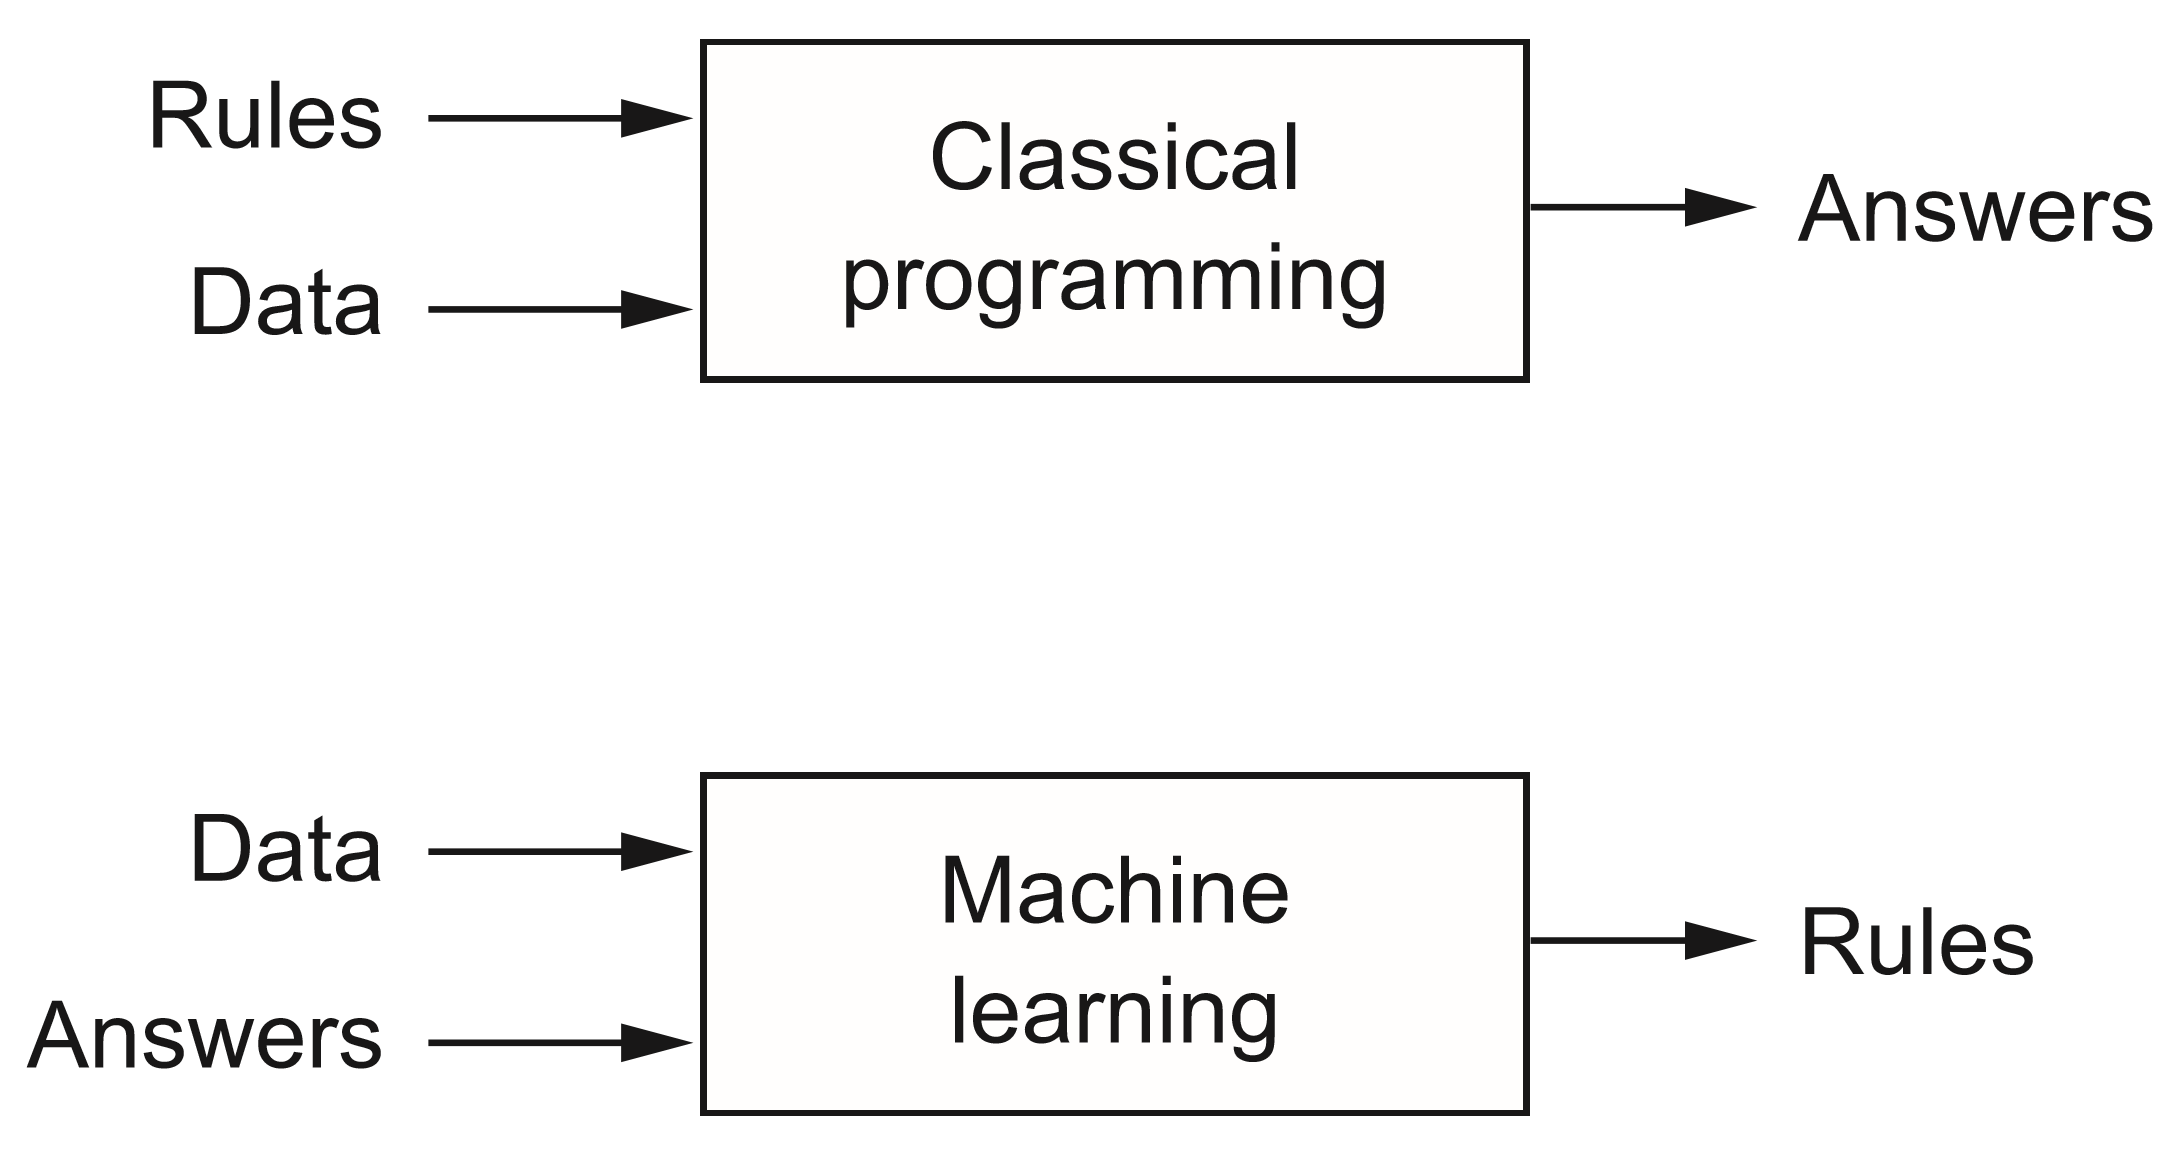
\includegraphics[width=0.5\textwidth]{images/classical_prog_vs_ml.png}
    \caption{Machine learning, a new programming paradigm, from
        \cite[p.5]{Chollet2017}}
\end{figure}

The promise made by machine learning is that the rules learned can be significantly more complex than it is feasible to program them by hand.
A good example for this is image recognition (which will be the focus of this project), in which the content of images is to be classified.
Relations between pixels have to be figured out resulting in a fairly complex model.
This is not feasible to program in traditional manner even for the simplest tasks.

The universal approximation theorem\cite{Cybenko1989}\cite{Hornik1989} states that for an arbitrary input $x$ there is a function $h$ approximating the mapping $y$, whereas the mapping is only the input to the respective correct output (often labeled by a human).
This relationship is shown in equation~\eqref{eq:universal_approx} \footnote{In literature there is often a bias inside the sum.
Following the convention to prepend a 1 to the input vector $x$, this is always included.
Please note that this is mathematically the same but just a matter of taste.
}
% TODO define sets X and Y of \theta and x
\begin{equation}\label{eq:universal_approx}
    \forall \epsilon > 0 :
    \exists h(\theta, x) : \forall x \in I : | h(\theta, x) - y(x) | < \epsilon
\end{equation}
% TODO the text here can be changed with a class of functions (see UAT paper)
The mathematical description of $h$ is called the model (e.g.  $h(x) = \sum_{i=1}^n{\lambda (\theta^T * x)}$).
$\lambda \in \mathbb{R}$ is a constant and $\theta$ is a tensor defining the parameters of $h$, composed of so called weights and biases. % TODO was biased already defined? ...
The universal approximation theorem makes no assertions over the shape of $\theta$; therefore $h$ is called the hypothesis, because it states that for a specific composition of $\theta$ this equation holds to be true.
This notion is summarized in equation~\eqref{eq:hypothesis}.

\begin{equation} \label{eq:hypothesis}
    \forall \epsilon > 0 : \exists \theta \in X : \forall x \in I : |
    h_\theta(x) - y(x) | < \epsilon
\end{equation}

For model evaluation a loss function is used; it compares the result of the hypothesis with provided data.
The most prominent loss function is called \name{mean squared error}.
It takes the sum of the deviation of $n$ examples squared and divides them by $2*n$.

\begin{equation} \label{eq:mse}
    L_{mse}(\theta, x) = \frac{1}{2 n} \sum_{i=1}^n (h_\theta(x) - y(x))^2\end{equation} 

The task of machine learning is to determine a $\theta$ for a model confirming equations~\ref{eq:universal_approx} and \ref{eq:hypothesis}, which is done by iteratively updating $\theta$. 
Before training $\theta$ is initiated randomly and then adjusted iteratively to let the $\epsilon$ converge to zero, thus minimizing the value of $L$.
% TODO find paper for random initialization... I have one.

For the loss function to gradually decrease $\theta$ is adjusted using an optimizer function which is famously done using gradient descent or some variant of it.
Gradient descent is performed by calculating the gradient of the loss function and subtracting it from the respective parameters, shown in equation~\eqref{eq:gradient_descent}.

\begin{equation} \label{eq:gradient_descent}
    \theta_{i+1} := \theta_i - \eta \nabla_\theta L(\theta, x)
\end{equation}

Herein $\eta$ is a constant, called the learning rate which helps the loss function to converge to 0 using gradient descent.
It is one of many hyper parameter which are not adjusted, but determined before training. An optimal setting of hyper parameters is an important task which is hard to automate and therefore focus of a lot of research\footnote{There are algorithms to adjust the learning rate, namely AdaGrad\cite{Duchi2010} and derived algorithms.}.
If equation~\eqref{eq:hypothesis} holds to be true for the model, it is going to be a sufficient fit for the given input.

Subsequently these concepts are introduced presenting a simple example.

\subsection{Simple linear example} \label{ch:simple_linear_example}
% TODO more descriptive title?

As an illustrative example a model translating Fahrenheit into Celsius will be created.
The original equation is given by the linear function $y = mx + b$ as $F = C * 1.8 + 32$, with $F$ as degree Fahrenheit and $C$ as degree Celsius respectively.

A model designed to learn this relationship is defined in listing~\ref{lst:c_to_f} \footnote{\url{https://klawr.github.io/deepmech/reports/srp/demos/c\_to\_f.js}} .

% TODO add JavaScript as language
\lstinputlisting[label={lst:c_to_f}, caption={Celsius to Fahrenheit}]{demos/c_to_f.js}

The model described has $\theta$ implemented through \code{w} and the hypothesis function by \code{h}.
Since we know that the relationship is linear, the model represents a one dimensional polynomial, using the first index as dimensionless (emulating the bias as previously mentioned) and the first as input x.
We will add one dimension later to demonstrate the behavior on polynomials which do not represent the target function immediately.

\code{y} provides the correct answer.
Please note that \code{y} is only used in training and can be omitted once the model parameters are properly adjusted.

In this example the loss function is described by the \textit{mean squared error } \footnote{ Abbreviated as \textit{mse} } which is shown in equation~\eqref{eq:mse}.

To minimize the loss function gradient descent described in equation~\eqref{eq:gradient_descent} is used.

In listing~\ref{lst:c_to_f} equation~\eqref{eq:gradient_descent} is implemented as \code{sgd} using $\theta_0 = \code{b}$ and $\theta_1= \code{m}$ as shown in equation~\eqref{eq:sgd_mse_here}.

\code{sgd} is short for \textit{stochastic gradient descent}.
\footnote{A distinction is made between batch, mini-batch and stochastic
    gradient descent;
    using the full data set, a defined subset or single inputs respectively on
    each iteration.}
It represents the optimizer function, updating the parameters of the model by taking the gradient of the loss for each individual parameter and updating them simultaneously.

\begin{equation} \label{eq:sgd_mse_here}
    \begin{split}
        \theta_{0} & := \theta_{0} - \frac{\partial L}{\partial \theta_{0}} =
        \theta_{0} - (h(x) - y(x))  \\
        \theta_{1} & := \theta_{1} - \frac{\partial L}{\partial \theta_{1}} =
        \theta_{0} - (h(x) - y(x)) * x
    \end{split}
\end{equation}

The respective output may look like:
\begin{lstlisting}
loss:  343041.666256673
loss:  16242.7707476548
loss:  88.27595280422442
loss:  10.74432403839251
loss:  1.1607137779951606
loss:  0.252186283500194
loss:  0.00040450626910586374
loss:  0.00004247033303206121
loss:  7.158429555712516e-7
loss:  1.6948019668728757e-10
weights:  [ 31.99999973758735, 1.8000003977458756 ]
\end{lstlisting} 

Expected behavior for the loss function is to decrease at every iteration, which it evidently does and thereby showing that the deviation of the hypothesis to the actual result is diminishing.
After iterating 200 times the parameters \code{m} and \code{b} of the \code{model} are logged and show that they are actually close to the anticipated result.
By increasing the iteration count, the result can be increased to the point where they are rounded to represent exact results (using Node.js\footnote{ As far as we can assume exact results using floating point numbers in computing.}).

\begin{SCfigure}
    \centering
    \caption{ The provided example may be visualized like this.
        The bias can be interpreted as an extra input which is always 1.
        The input is multiplied by the parameters labelling their respective arrows, which are in turn summed up (resulting in $y = mx + b$) }
    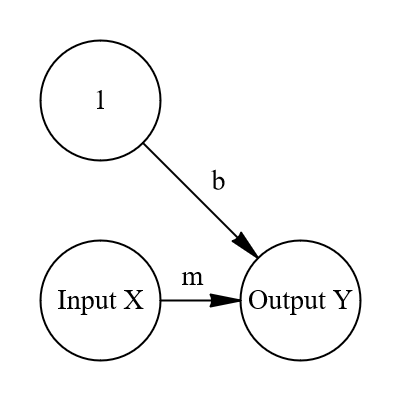
\includegraphics[width=0.4\textwidth]{images/1_simplest_nn.png}
\end{SCfigure} 

Provided this hypothesis is initially well suited for the task, it is important to note that by modify the hypothesis to represent a polynomial of a higher degree (e.g. $y = nx^2 + mx + b$) the extra parameters are converging to zero, effectively providing the same result as before
\footnote{But to achieve similar results the iteration count has to be increased by at least a factor of 20.
You can review the experiment at \url{https://klawr.github.io/deepmech/reports/srp/demos/c_to_f_adv.js}}.
